%%==========================
%% chapter01.tex for TJU Master Thesis
%% based on CASthesis
%% modified by charlie.yaha@gmail.com
%% version: 0.1alpha
%% Encoding: UTF-8
%% last update: Dec 5th, 2010
%%==================================================

%\bibliographystyle{TJU} %[此处用于每章都生产参考文献]


\chapter{绪~论}


\section{研究背景}

液压系统是航空航天等产品的重要系统。而液压系统的各类管线,是现代航空航天工业中极为重要的部件,对其可靠性的要求仅次于发动机。
本文的研究对象就是其中的软管组件。


现代飞机航面操纵系统与动力收放系统几乎都是液压驱动的。液压系统作为飞机飞行控制系统和起落架等负载的动力源,对飞机的安全飞行起着关键的作用。
大型客机的液压系统,是一个多余度、大功率的复杂综合系统,控制着飞机起落架、襟翼、减速板的收放,平尾、副翼、方向舵的操纵,进气锥、辅助进气门的调节等\cite{dingfei2010}。空客的A320,波音的B737都配备了至少3套相互独立的液压\cite{dingfei2010},多套液压系统相互独立、相互备份,管线密布机身,如图\ref{fig:plane-hose}所示,管线长度一般在机身长度的数倍以上。




\begin{figure}[!htbp]
	\centering
	\subfigure[机身软管管路(a.软管,b.液压源)]{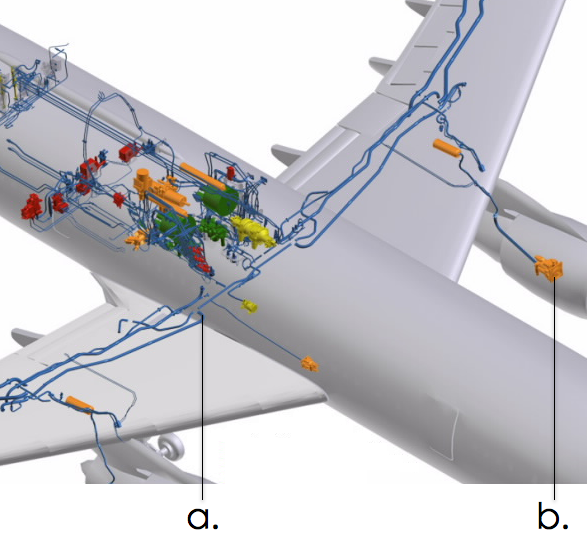
\includegraphics[width=0.4\textwidth]{figure/chap1/plane-cruit}\label{fig:plane-cruit}}    
	\hspace{1cm}
	\subfigure[发动机软管管路(a.软管,b.液压源)]{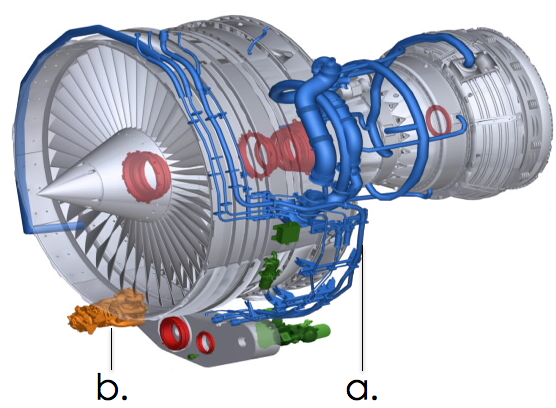
\includegraphics[width=0.4\textwidth]{figure/chap1/engine-cruit}\label{fig:engine-cruit}}    
	\fcaption{飞机液压软管管路}{Cruit system of Hose Assembly}
	\label{fig:plane-hose}
	
\end{figure}




据统计,当前我国飞机液压系统的故障几乎都发生在管路部分,
而液压系统的故障约占飞机机械系统总故障的左右$1/3 $,飞机液压系统的维修工作量占机械维修工作量的$ 30\%$\cite{lijun2007},
液压软管的可靠性问题是飞机故障、事故的主要原因之一。

液压管路的泄漏、失效往往是由液压泵的压力脉动引起的。现代飞机液压系统大多采用变量柱塞泵,脉动式的流量输出是其固有特性;同时液压系统工作时,在阀门打开或关闭的瞬间,供压管路和回油管路会出现强烈的压力撞击,即压力脉冲。变量柱塞泵产生的压力脉动,在高速、高压、高温、大流量条件下,若与系统匹配不当,油泵出口压力会产生高频等幅振荡,从而很容易导致两种耦合振动:一种是脉动频率与流体谐振频率接近时的耦合振动;另一种是脉动频率与管路系统结构的固有频率接近时,发生的耦合振动。
在高压管路上,压力脉冲峰值有可能达到系统额定压力的1.5倍以上,而在回油管路上则可能达到正常回油压力值的10倍以上\cite{lijun2007}。
这种脉冲峰值很容易导致管壁破裂、管路支撑结构破坏,引起支撑刚度下降、管路系统失效、液压油液泄露,从而导致严重的灾难性事故\cite{gaofeng2013}。


例如,我国七十年代研制的某机型,从油泵出口至蓄压器之间的软管管路不断发生断裂,影响到设计定型;
八十年代初,我国研制的某型号机地面试车时,由于液压软管爆裂引发大火,致使整架飞机毁于一旦,不仅造成巨大的经济损失,还使型号研制进度推迟了两年;某型机的泵出口软管出现多次爆裂事故,由于管路断裂,液压系统失效,发生了飞机启用应急系统、强迫着陆及驾驶员应急跳伞等严重问题\cite{lijun2007,guoqing2010,gaofeng2013}。

\begin{figure}
	\centering
	\subfigure[波音b777起落架液压软管]{
		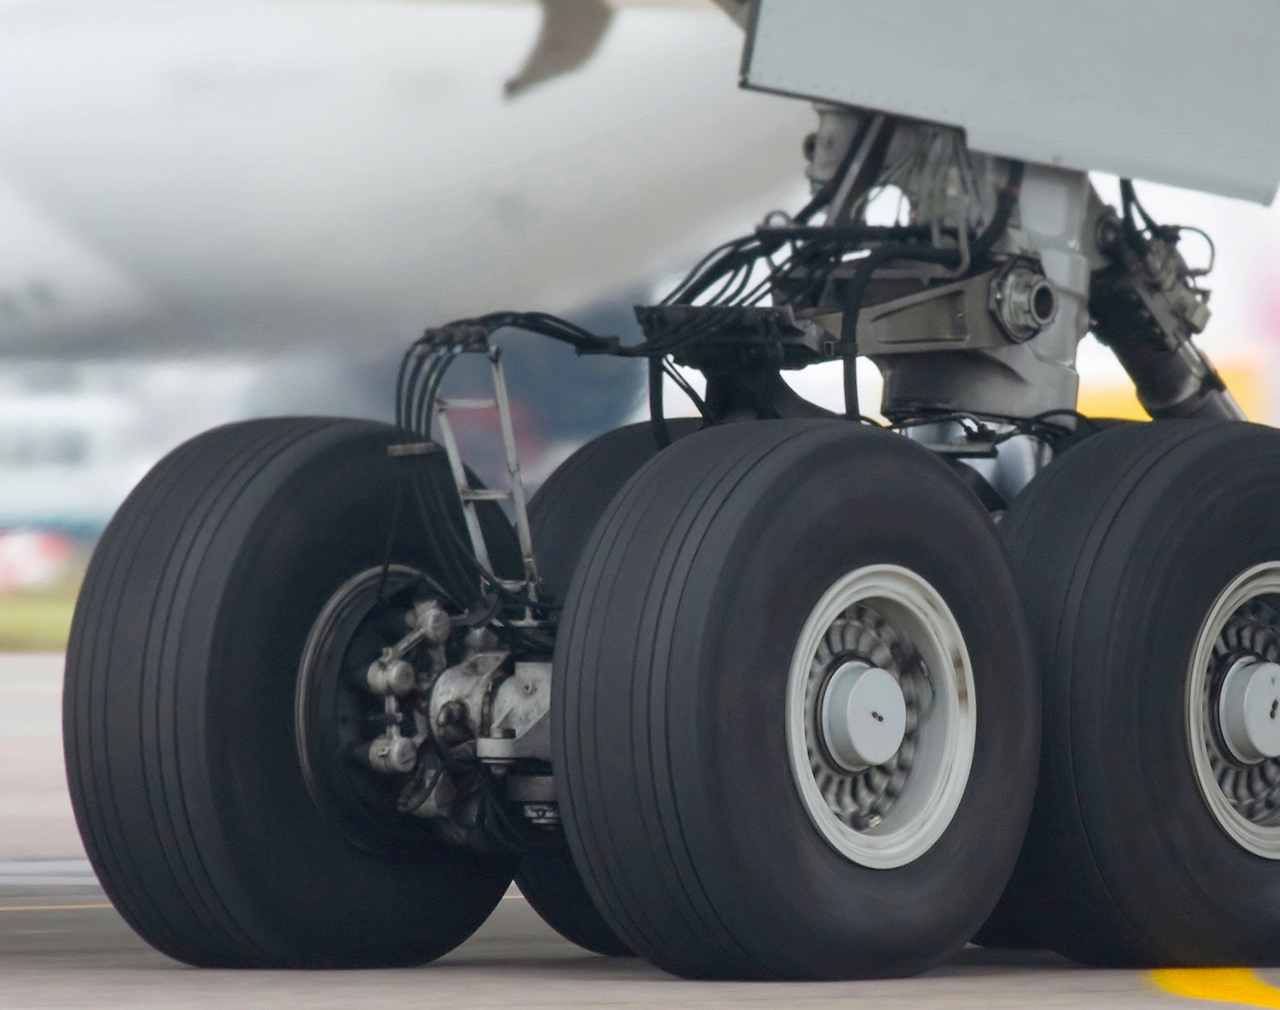
\includegraphics[width=0.4\textwidth]{figure/chap1/777-gear}\label{fig:777-gear}}
	\hspace{1cm}
	\subfigure[a380起落架液压软管]{
		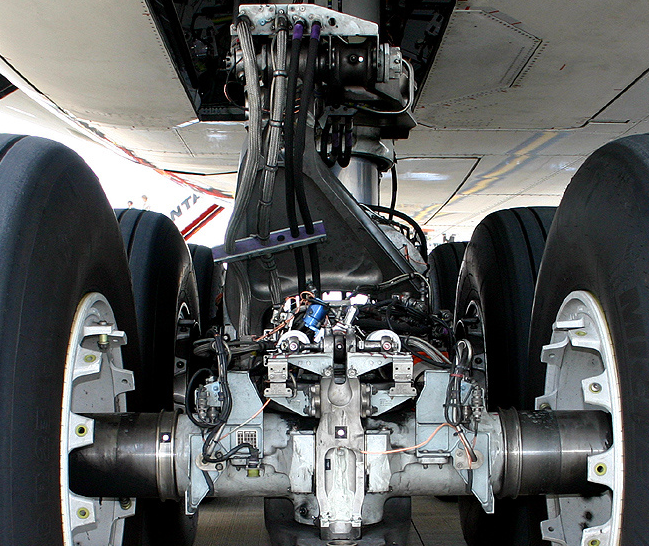
\includegraphics[width=0.4\textwidth]{figure/chap1/a380-gear}\label{fig:a380-gear}}
	\fcaption{起落架软管管路}{Hydraulic hose cruit of gear}{}
	\label{fig:plane-hose-2}
\end{figure}

因为液压泵出口处的高频振动,刚性管受激共振而破坏失效,必须要低刚度的柔性管来吸收振动的能量,
同时因为飞机液压能源系统由于飞机对空间和质量的限制,常常具有一般管路设计中需要避免的长跨度、低刚度管段出现\cite{gaofeng2013}。
因此,飞机动作控制液压系统(\ref{fig:plane-cruit})以及飞机引擎液压、燃油系统(\ref{fig:engine-cruit})中,大量的管道并非刚性管,而是由大量柔性软管组成的。


随着航空技术的不断发展,飞机液压系统也在向高压化、大功率的方向发展。
因为提高飞机的液压系统工作压力是减小系统自身重量和体积的重要手段。
空客A320液压系统额定工作压力为3000psi(21MPa)
最新的客机型号波音的B787和空客A380的液压系统压力等级都达到 5000psi(35MPa)\cite{lavooij1991},
国外领先企业Eaton Aerospace、Parker Hannfin公司也已经为军用飞机开发出来8000psi(55MPa)的液压泵,空客公司也已经提出了将起落架刹车制动液压管路工作压力提高到8000psi(55MPa)的目标,而国内的液压系统一般只能做到3000psi(21MPa)。


\begin{figure}
	\centering
	\subfigure{
		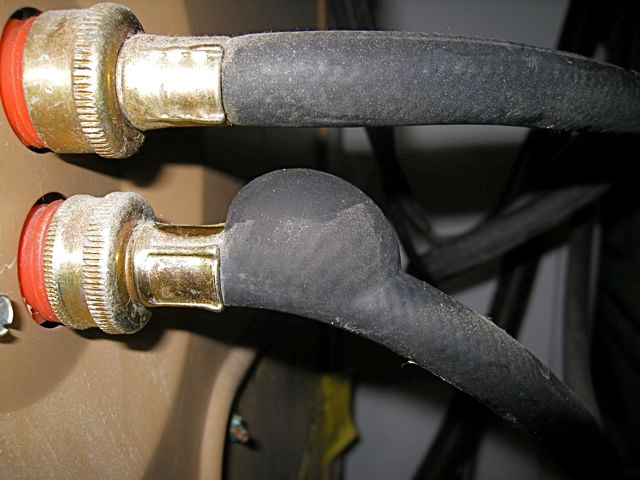
\includegraphics[width=0.3\textwidth]{figure/chap1/burst-hose-1}}
	\hspace{1cm}
	\subfigure{
		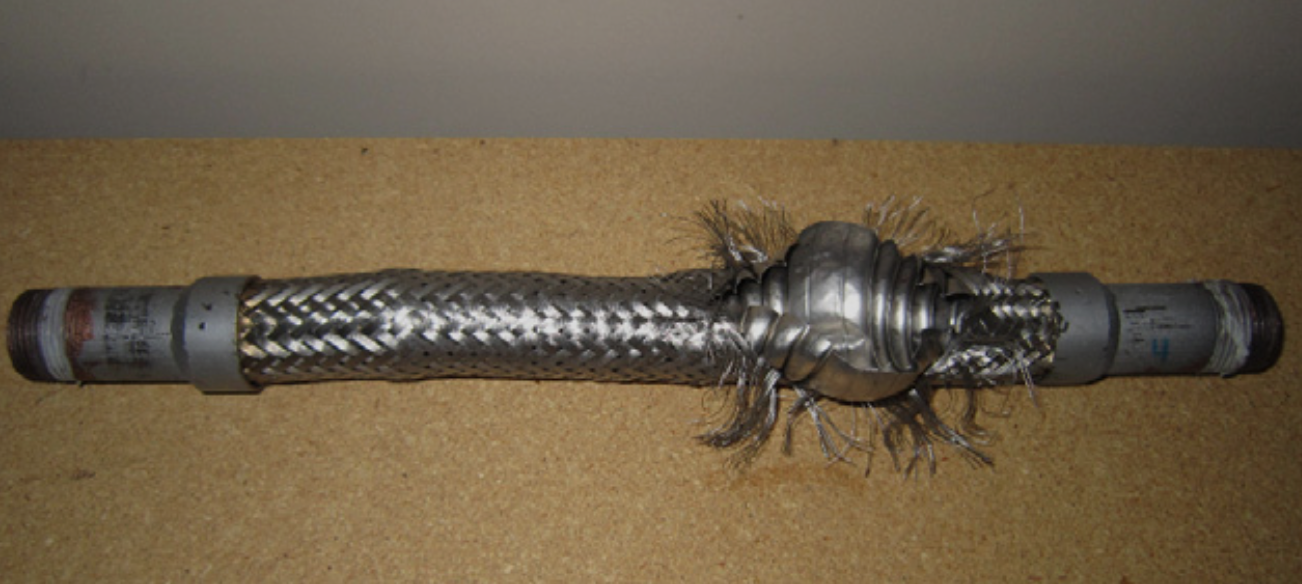
\includegraphics[width=0.5\textwidth]{figure/chap1/burst-hose-2}}
	\fcaption{软管失效形式}{ Failure Modes of Hose Assembly}
	\label{fig:hose fail}
\end{figure}





液压泵脉动控制方面,国内液压泵一般流量脉动为$\pm10\%$,国外一般在$ \pm5\% $左右\cite{lijun2007}。Eaton公司为空客A380最新研制出一种内置衰减器的柱塞泵,压力脉动变化为$ \pm 1\%$。可见国内液压泵脉动控制的水平与国际先进水平差距较大,考虑到新型柱塞泵的研发周期,这种差距短期之内很难弥补。
而飞机液压系统的压力脉冲是造成液压管路提前损坏,导致液压系统故障的主要原因之一。这就对我国液压管路的设计、生产水平提出了更高的要求。





%了解什么事软管
\section{软管组件简介}
%软管定义,软管组件结构

在因为在实际工程环境中,特别是各类飞行器中,很多情况下刚性管无法使用,b包括:1)液压元件持续的运动,2)液压元件任意或不规则排列,3)安装空间不足
4)管路剧烈振动,
5)管路受到冲击,
6)管路区段有高压力的释放。
为了克服以上不利条件,一般采用柔性的液压软管。这种柔性液压软管是一种复合结构的管路连接件,一般将整个系统结构称为软管组件(Flexible Hose Assembly),或软管总成(本文统一称为软管组件)。





其结构包括了柔性内管、加强层、保护层,以及金属连接件。
柔性软管的材料一般为橡胶管,氟塑料管,热塑料管,金属波纹管等;内管外包覆若干层加强结构,如编织、缠绕等。
软管组件工作时,绝大部分内压荷载由加强层承担,内管主要起通道的作用。加强层数一般视内压荷载大小而定。


\begin{figure}[!htbp]
	\centering
	\subfigure{
		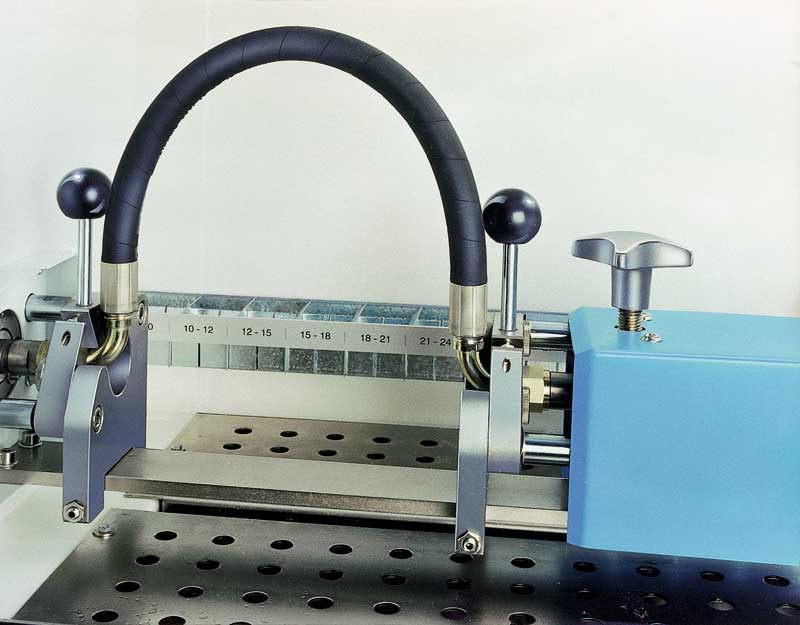
\includegraphics[width=0.45\textwidth]{figure/chap1/hose1}}
	\hspace{0.5cm}
	\subfigure{
		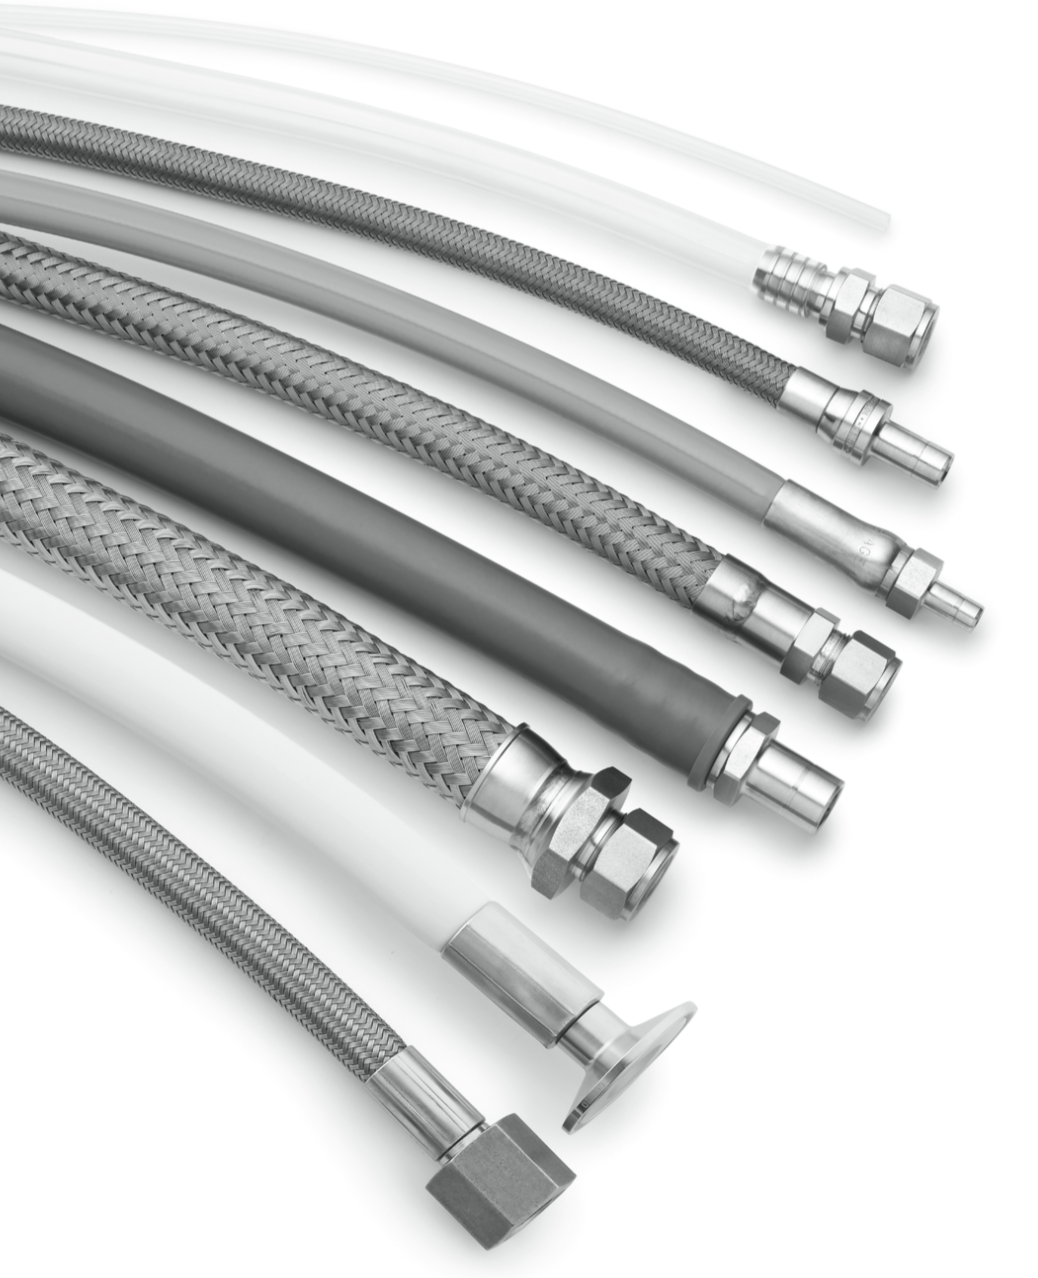
\includegraphics[width=0.3\textwidth]{figure/chap1/hose2}}
	\fcaption{常见软管组件}{Usual Forms of Hose Assembly}  
	\label{fig:hose}
\end{figure}


软管组件同时也应用于气动、燃油、滑油等系统的介质传输,起到了“血管”作用,航空航天飞行器、汽车、船舶,以及各种工业设备、机床等,都大量使用了软管组件。相比普通硬质管,软管组件可以承受相对较大的内压、轴向荷载,同时保持较小的质量、弯曲刚度,带来以下优势:可以减小系统的刚度,吸收液压源产生的振动;安装方式灵活,节约了系统内部的空间。




%软管优势



%不同软管型号
软管组件根据不同的压力等级可以分为低压、中压、高压、超高压几种型号,如表\ref{tab:hosepressurelevle}所示,





\begin{table}[!htbp]
	\centering
	\tcaption{软管组件压力等级}{Hose Assembly Pressure level}
	\label{tab:hosepressurelevle}
	\begin{tabular*}{0.6\textwidth}{@{\extracolsep{\fill}}>{\hspace{0.5cm}}ccc}
		\toprule
		    &   英制 / psi   &  公制 / MPa  \\ \midrule
		低压  & $ \left[ 1000 , 3000  \right)  $&  $ \left[ 0 , 7  \right)  $  \\
		中压  & $ \left[ 1000 , 3000  \right)  $&  $ \left[ 7 , 21  \right)  $ \\
		高压  & $ \left[ 3000 , 4000  \right)  $&  $ \left[ 21 , 28  \right)  $ \\
		超高压 & $ \ge$4000 &  $ \ge$28  \\ \bottomrule
	\end{tabular*} 
\end{table}

根据美国\footnote{SAE AS1946,SAE AS604,SAE AS1339}、欧洲以及国际标准化组织\footnote{ISO1436,ISO3862
}的安全标准,软管组件的脉冲安全系数为$ 4:1 $,
即软管组件受压力脉冲破裂时,所使用的真实压力需达到4倍额定压力,一般将该压力值定义软管组件的爆破压力。
因此,低压软管的爆破压力一般在以下30MPa;目前国内3000psi液压系统配套的软管组件,其爆破压力至少为85MPa;国际新一代大型客机已经要求软管组件爆破压力至少为140MPa。


根据软管组件内管管径的不同,可以分为轻型、中型、重型,
管径在6mm以下的一般归为轻型管,管径14mm以上的为重型管。

根据不同的工作压力、流量的需求,各型软管的常见用途如表\ref{tab:hosefixposition}所示,

\begin{table}[!htbp]
	\centering
	\tcaption{不同型号软管组件安装位置}{Position}
	\label{tab:hosefixposition}
	\begin{tabular*}{0.8\textwidth}{@{\extracolsep{\fill}}>{\hspace{0.5cm}}ccc}
		\toprule
		&    轻型     &     重型     \\ \hline
		低压 & 汽车刹车、转向传动 &  输运水、气  \\
		高压 & 飞机起落架、襟翼  & 飞机、船舶液压泵出口 \\ 
		\bottomrule
	\end{tabular*} 
\end{table}

%解释表格
飞机、船舶液压泵出口处压强高,流量大,震动强,工作环境极为恶劣,因此国内外一般都采用重型高压软管组件,技术也都较为成熟。
飞机起落架、襟翼等部位处于机身液压系统的末端,但压强仍然很高,而且软管的安装空间很小,要求软管组件具有较小的弯曲半径。保持较高的爆破压力的同时,使得软管组件小型化、轻型化,这就对软管组件的设计水平提出了很高的要求。国外企业在轻型高压软管组件领域技术优势明显,基本垄断了该市场。
以飞机液压系统高压化的趋势,我国在这一领域的短板会更加明显的凸显出来。而这一型的软管组件,仅仅依靠看经验仿制已经很难实现,对科学可靠的设计理论的探求已迫在眉睫。

汽车领域也大量使用了软管组件,例如刹车制动管,转向传动管,空调管等。相比飞行器的液压系统,汽车的液压系统压强较低,如刹车制动管的爆破压力一般为35MPa至40MPa\footnote{GB 16897-2010}。但汽车行业对成本较为敏感,要求在保证设计指标的同时,使软管的结构达到最优化。这对软管的设计、制造也提出了很高的要求。

 	 	 
\section{软管组件加强层研究现状}		


%目前对金属编织加强软管的研究,多见于汽车工业中的中刹车管[2]、转向传动管[3]、空调管[4] 等。

软管组件作为一种20世纪中叶就开始广泛使用的重要工业构件,
对其加强层的研究一直以实验、实用为主,没有形成一套通用完整的体系。这与软管组件的发展历史有着密切的联系。


\subsection{软管工业发展历史及行业现状}

软管组件的加工生产技术经过几次重大变革,至今为止,已经发展出了3代产品,主要是以软管组件的加强层结构、材料来划分的。

金属高密度编织增强软管组件是由美国发明并于20世纪60年代开始用于飞机的液压系统,
%第一代
在此之前为第一代软管组件,以橡胶软管为主,可以追溯到19世纪80年代\cite{Breig1988};

从上世纪60年代到上世纪90年代中期,
第二代金属加强软管已经广泛应用于航空、航天领域。同时也根据不同的压力等级需求和工作环境发展出不同的加强形式,如编织加强、缠绕加强;也发展出了不同的内管材料,如PTFE氟塑料、热塑料、尼龙等;还出现了防火、防磨损、防腐蚀、防紫外线等各式附件,品种繁多。
为此,美国建立了一系列的军用、宇航产品技术标准或规范,例如:MIL-H-25579E、SAE AS604、SAE AS614等。
第二代软管组件的最高使用温度已达232\textcelsius,最高工作压力已经达55MPa,
已经广泛应用于各种类型的飞机和导弹、运载火箭等。

%第三代
近年来,航空航天事业飞速发展,对软管组件也提出轻量化的要求,传统钢丝增强软管组件已不能满足航空航天的设计要求。
为了解决这个问题,美国Titeflex、Eaton及Parker等国际知名公司,已在20世纪80年代,开始了非金属增强软管组件的研究,也就是第三代软管组件。他们纷纷研制推出了各自的非金属增强软管组件产品。目前波音B787就大量使用了Eaton公司的AS1975以及AS4623 Kevlar加强软管组件,满足5000psi(35MPa)工作压力要求。

\begin{figure}[!htbp]
	\centering
	\subfigure{
		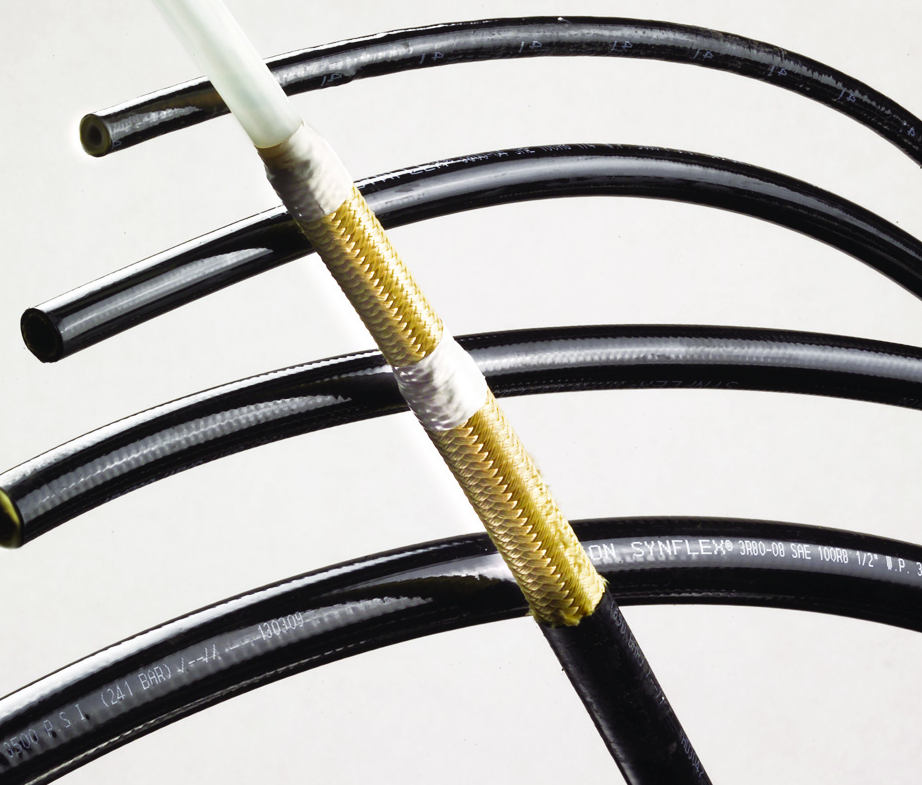
\includegraphics[width=0.3\textwidth]{figure/chap1/kevlar-hose}}
	\hspace{0.5cm}
	\subfigure{
		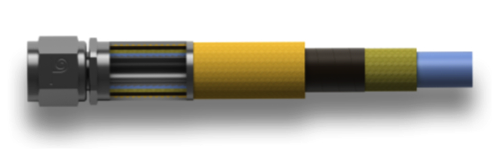
\includegraphics[width=0.5\textwidth]{figure/chap1/kevlar-hose-2}}
	\fcaption{Kevlar加强软管组件}{Kevlar Reinforced Hose Assembly}  
	\label{fig:kevlarhose}
\end{figure}


我国目前钢丝增强液压软管年产量约6000万米\cite{xuhaitao2013},但大多为低端低压产品。
尚未出现非金属纤维增强的软管组件,都属于第二代金属纤维增强的范畴。相对较为先进的国产软管组件也只达到了5000psi(35MPa)。并且国内尚无航空软管的相应标准,没有成熟的规范、标准实验设施和完整的实验方法。可以说国内软高端管组件行业还处于起步阶段,距离轻量化,标准化,高压化的国际水平还有不小的距离。



\subsection{加强层理论分支及现状}
针对软管组件的研究有两个比较明确方向:1)加强层的力学行为和力学本构;2)连接件与管体的扣压工艺过程。
软管组件的接头连接技术是一个非常重要的研究方向,
但本文的研究主要针对加强层,这里不对软管组件的连接技术进行阐述。这里主要介绍加强层理论分支及现状。


对软管组件加强层的理论的研究主要还是由行业的需求驱动,不同的几代产品并不是一个相互取代的关系,而是在不同领域不同需求并存的关系。几种不同材料,不同结构的加强层形式,使得该领域的研究出现了几个分支。图\ref{fig:hose-system-theories}描述了软管组件加强层的理论路线和分支。


\begin{figure}[!htbp]
	\centering
	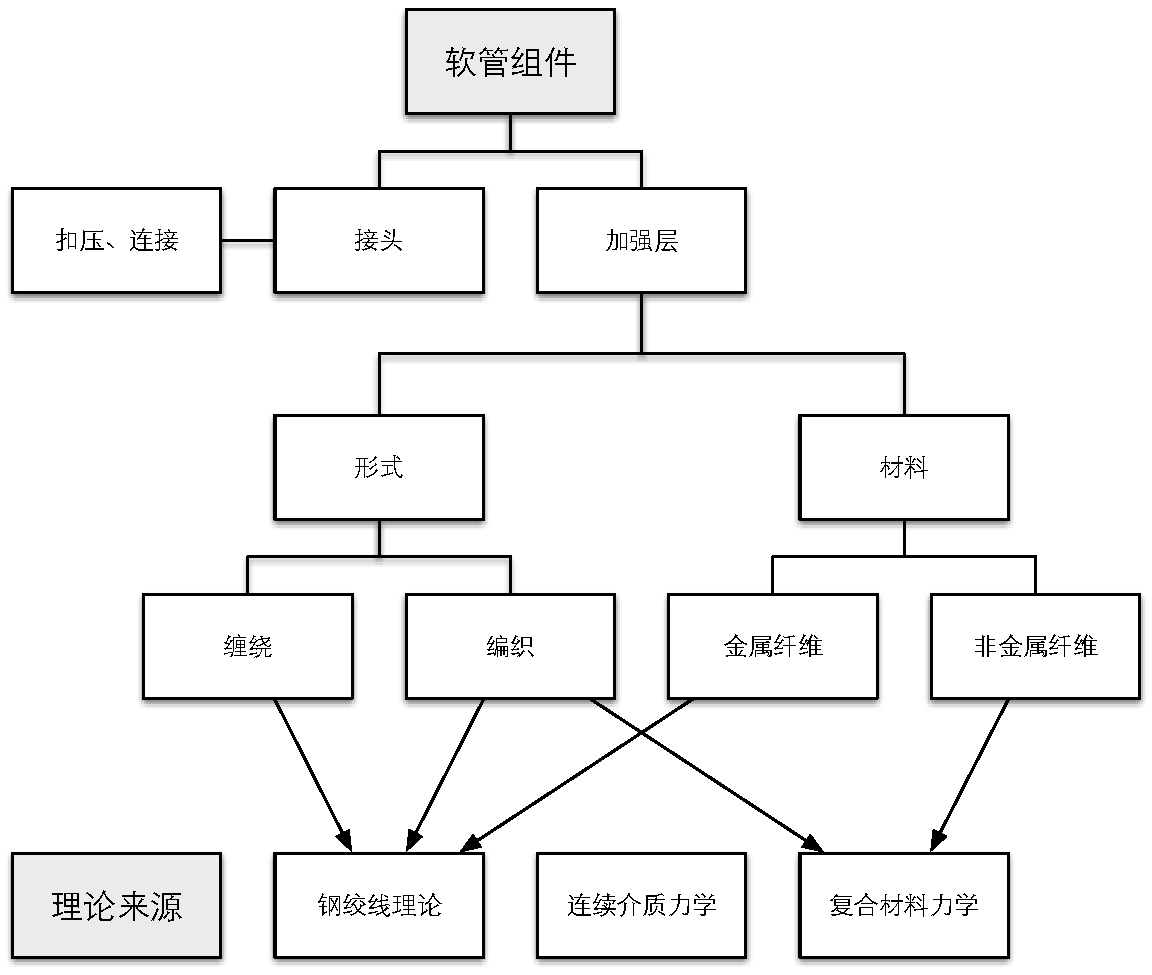
\includegraphics[width=0.7\linewidth]{figure/chap3/理论体系}
	\fcaption{软管组件理论体系}{Hose Assembly Theory Branches}
	\label{fig:hose-system-theories}
\end{figure}



加强层的理论研究成果,根据本文对国内外文献成果、专利、标准等的调研情况,主要是从两个理论体系发展而来的,包括了
\begin{inparaenum}[1)]
	\item 钢绞线理论;
	\item 复合材料力学。
\end{inparaenum}
还有一小部分研究采用了连续介质力学的观点与研究方法。几个理论分支对于编织与缠绕,金属纤维与非金属纤各有侧重。

%如图\ref{fig:hose-system-theories}所示,一般采用金属纤维的缠绕层会沿用钢绞线理论的分支,理论结合工程经验,效果令人满意;金属纤维编织层


\subsection{基于钢绞线理论的研究}

基于钢绞线理论的主要针对金属纤维缠绕的加强形式。将各股纤维缠绕在一起,加强多股纤维的整体性,如图\ref{fig:helical-strands}所示,这种螺旋绞合的结构(Helical Strands)多用于主要用于大桥的悬索和输电线的加强。钢绞线理论应用于加强层的力学分析,始于20世纪50年代,包含了两个分支\cite{Evans2002}:
\begin{inparaenum}[1).]
	\item 加强层含量较低,橡胶管起主要作用的软管,由\citeauthor{Kuipers1989}等人\cite{Kuipers1989,Horn1988}提出并完善,一般适用于第一代软管组件,例如帘线加强的软管;
	\item 加强层主要承力的软管,主要研究的是高密度钢丝缠绕加强层。第二代软管组件以这套理论指导设计。
\end{inparaenum}
这套理论体系成熟与上世纪90年代初,适用于金属纤维的缠绕层,编织层仅仅被作为缠绕层的一种扭转为0的特殊情况\cite{Breig1988}。



\begin{figure}[!htbp]
	\centering
	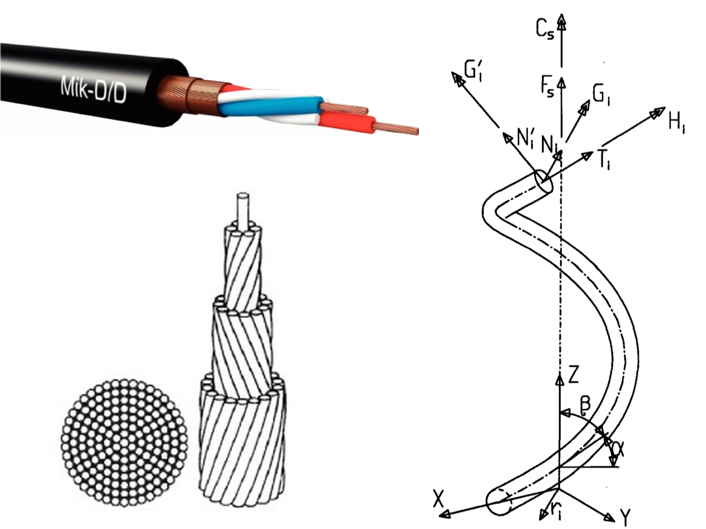
\includegraphics[width=0.6\textwidth]{figure/chap1/helical-strands}
	\fcaption{螺旋绞线}{Helical Strands}  
	\label{fig:helical-strands}
\end{figure}



%stepI hruska 
\citeauthor{hruska1951calculation}\cite{hruska1951calculation,hruska1952radial,hruska1953tangential}分析了钢绞线结构中一层钢丝的轴向、切向以及径向的应力。钢绞线中一层钢丝实际上就是一层螺旋缠绕结构,也被用于早期设计软管组件缠绕层的参考依据。而其理论并没有考虑结构半径的变化,也没有考虑钢绞线排布的角度$ \alpha_i $的变化。也就是说,该理论不能考虑编织层受内压后,结构的几何变化。该理论仅考虑了钢绞线的拉伸刚度,扭转和弯曲的刚度皆为0。钢绞线体系轴向拉力$ T_\alpha $与单根钢丝轴线拉力$ T_i $的关系为:
\begin{equation}
T_\alpha = T_i \cos{\alpha_i}
\end{equation}

1951年,\citeauthor{hruska1951calculation}也给出了单位长度径向力$ F_{RU} $与钢绞线拉力$ T $、钢丝曲率半径$ \rho $关系的表达式,如式\ref{eq:Hruska}所示。该理论提出时仅作为实验得到的经验公式,后在\citeyear{machida1973}年由\citeauthor{machida1973}\cite{machida1973}给出证明。

\begin{equation}\label{eq:Hruska}
{F_{RU}} = \frac{T}{\rho }
\end{equation}
其中,钢丝的曲率半径可以由螺旋缠绕的结构参数表征
\begin{equation}
\rho  = \frac{R}{{{{\sin }^2}{\alpha _i}}}
\end{equation}
$ R_i $为钢绞线总体半径。


1977年,\citeauthor{Entwistle1977}\cite{Entwistle1977}针对编织加强软管,提出了一套更为准确的理论假设。这套理论相对之前的理论,可以考虑缠绕层受内压荷载后,结构的几何变化。\citeauthor{Entwistle1977}对加强层几何变化的假设如图\ref{fig:assumption-deformed-geometry}所示,该理论不允许软管发生扭转,这是考虑到在该理论体系下编织层的扭转必须为0。

加强层变形前后的半径为$ R_i $、$ R_i' $,缠绕角为$ \alpha_i$ 、 $\alpha_i' $,钢丝应变为$ \varepsilon_i $,之间的关系可以通过图\ref{fig:assumption-deformed-geometry}中的几何关系表示

\begin{equation}
\frac{{{R_i}'}}{{{R_i}}} = \left( {1 + {\varepsilon _i}} \right)\frac{{\sin {\alpha _i}'}}{{\sin {\alpha _i}}}
\end{equation}

\begin{figure}[!htbp]
	\centering
	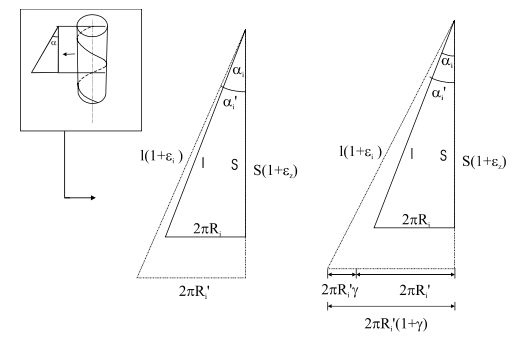
\includegraphics[width=0.7\linewidth]{figure/chap3/review/a}
	\fcaption{加强层几何变化假设}{Assumption of the deformation of  Reinforcement Layer}
	\label{fig:assumption-deformed-geometry}
\end{figure}

1979年,\citeauthor{Knapp1979}\cite{Knapp1979}针对内芯可压缩的钢绞线结构进行了研究,采用了和\citeauthor{machida1973}(\citeyear{machida1973})相似的手段,引入了扭转因子$ \gamma_i $(图\ref{fig:assumption-deformed-geometry}),其表达式为:
\begin{equation}
{R_i}' = {R_i}\frac{{\left( {1 + {\varepsilon _i}} \right)\sin {\alpha _i}'}}{{\left( {1 + {\gamma _i}} \right)\sin {\alpha _i}}}
\end{equation}

钢绞线理论体系下的研究,实际上还是围绕着加强结构中的钢丝本身,没有一个平均化的概念,所得的结果也是加强层中的某根钢丝与结构整体位移、扭转的关系。而且该系列理论主要研究的是缠绕加强,编织总是被简化为特殊的缠绕。编织远比缠绕来得复杂,很多复编织层特有的复杂关系、结构都被过度简化\cite{Breig1988}。

螺旋钢绞线中的钢丝纤维直径一般较大,因而不能忽略钢丝的扭转刚度。
在这种理论体系下,讨论钢丝加强层的力学性能时,往往更加关注钢丝本身的力学行为。这种钢绞线结构(Helical wound assembly)由于结构的复杂性,形成了一套独特的基于实验和经验的理论体系\cite{Cardou1997}。虽然有学者尝试用弹性力学推导理论解\cite{phillips1972,machida1973},但主要仍以经验公式为主。

软管组件的加强层一般采用较细的钢丝,比较类似于复合材料中的纤维,仅在金属丝轴向可以承受拉伸荷载。但是当时复合材料力学并未充分发展,因而软管组件沿用了螺旋钢绞线的理论,主要研究缠绕的加强方式\cite{Entwistle1977,Knapp1979},将编制作为一种特殊的缠绕方式来研究\cite{Breig1988}

传统的编织和缠绕理论是将各层编织角和缠绕角均设计为$  {\alpha _b} = {\tan ^{ - 1}}\sqrt 2  = {54.74^ \circ }$,
这个角度是从通过柱状薄壁容器理论推导得出的,使得单层金属缠绕液压软管轴向和环向受力平衡。
但是对于多层加强软管组件,这种中性角度下钢丝在受内压时变形较大、钢丝间应力损失大\cite{Evans2002},不能发挥每根钢丝的最大强度,但对像高压软管这种多层增强的厚壁管体,这个角度就很不适用了。比如按这个角度设计的软管,一个工作层其爆破压力可达理论值的80\%左右,两个工作层约75\%,三个工作层只有65\%左右,四个工作层或小口径的三个工作层,要达到50\%都有一定困难\cite{tangxi1994}。各增强层受力不均,内层应力大,外层应力小,且逐层递减。在脉冲实验和实际使用中,内层钢丝常因疲劳而断裂,中层和外层却完好无损,严重影响;对于编制加强软管组件,钢丝之间的相互影响更为复杂,传统的编织平衡角理论不能很好地反映出这种区别。有文献研究了多层钢丝增强软管内压、应力与变形的综合的动态平衡体系\cite{tangxi1994,Evans2002}。也有利用计算仿真软件来分析各层钢丝角度的组合形式对软管受力的影响是一种有效的方法\cite{zhubowei2010}。 

%在连接件扣压的方向,早期研究较为少见,近年来,随着数值仿真手段的发展,学者也对液压软管总成连接质量的影响因素进行了研究,分析了扣压工艺、接头形式如芯子和外套的结构等因素对软管总成连接质量的影响。建立了分析模型,分析了扣压力、扣压量的大小对软管总成连接质量间的关系,并对扣压过程进行了控制。

\subsection{基于复合复合材料理论的研究}


随着符合材料力学的发展,近30年来,大量学者对平面织物复合材料进行了研究。第三代非金属加强软管组件的理论,多来自于这类研究的成果。
\citeauthor{Tan1997}\cite{Tan1997},
\citeauthor{cox_handbook_1997}\cite{cox_handbook_1997},以及
\citeauthor{ko_three-dimensional_1989}\cite{ko_three-dimensional_1989}
对平面织物复合材料的本构模型进行了综述,通过他们对各类模型的归纳,可以发现,织物复合材料最主要的结构类型有\cite{Goyal2005}:
\begin{inparaenum}[1).]
	\item 纺织(Weaving);
	\item 编织(Braiding)。
\end{inparaenum}
其区别在于:纺织由经线(Warp)与纬线(Weft)正交穿插交叠而成;编织中的各股纤维不需要正交穿插,因此各股纤维间的相互作用更加复杂。
纺织一般只能平面的复合材料;编织可以形成管状的结构,传力方式也比平面结构更为复杂。
以上原因导致针对织物复合材料的模型,大部分是适用于纺织结构的,针对编织结构的只有较少的一部分。适用于管状编织结构的模型几乎没有\cite{Tan1997}。


1986年, \citeauthor{ma_elastic_1986} \cite{ma_elastic_1986} 针对编织纤维结复合材料提出了三维本构模型“对角单元模型”(Diagonal Brick),如图\ref{fig:diagonal}所示,代表了纤维的简化“特征单元”,包含了四个对角杆单元,代表了单元中纤维的取向;单元空间包含了材料的树脂。然而该模型并没有考虑纤维的弯曲,而这种弯曲应该发生在单元的顶点处;该模型同时也有考虑两股纤维交叠的截面\cite{whitney_modeling_1989}。有研究认为\cite{du1993unit},纤维含量超过0.5,4个对角线方向的纤维杆单元建模。


\begin{figure}
	\centering
	\subfigure[对角单元模型]{
		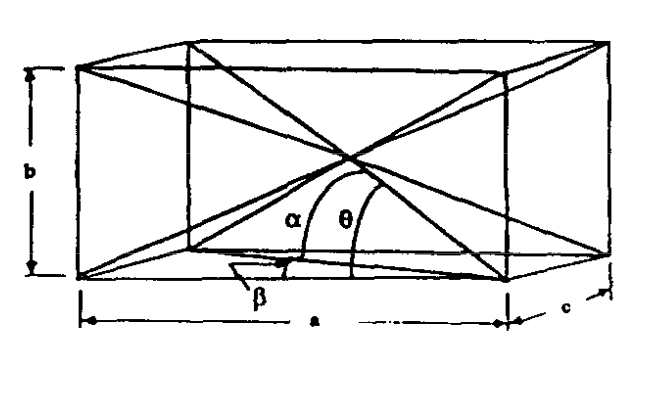
\includegraphics[height=0.12\textheight]{figure/chap1/diagonal}
		\label{fig:diagonal}
		}
	\hspace{1cm}
	\subfigure[倾斜纤维模型]{
		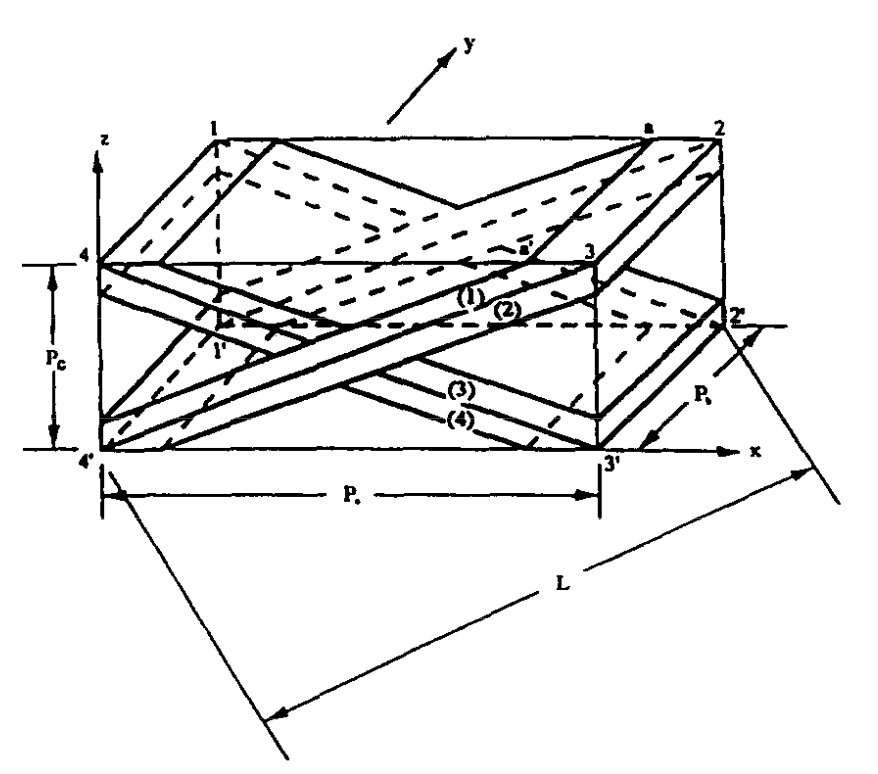
\includegraphics[height=0.2\textheight]{figure/chap1/fiber-inclinatino}
		\label{fig:fiber-inclinatino}
		}
	\fcaption{编织织物复合材料理论模型}{Models of Braided Composites}
	\label{fig:Models-of Braided-Composites}
\end{figure}





\citeauthor{yang_fiber_1986}\cite{yang_fiber_1986}发展了层合板理论,来研究三维编织复合材料。他提出了一个新的模型“倾斜纤维模型”(Fiber Inclination Model),将编织的单元视为几组倾斜单向层合板的组合,其特征单元如图		\ref{fig:fiber-inclinatino}所示。其中,倾斜的层合板代表了4股对角线方向的纤维。而该模型是对
\citeauthor{chou_one-dimensional_1983}提出的“起伏纤维模型”\cite{chou_one-dimensional_1983}的扩展,
其模型的预测与其他学者的实验能够较好的符合
\cite{florentine_magnaweave_1984,macander_fabrication_1986,gause_mechanical_1983}。但是以上的模型并不能很好的与实际编织的几何参数联系起来,并不能知道编织结构的参数优化。

\citeauthor{byun_analytical_1991}\cite{byun_analytical_1991}提出了一种利用几何模型,采用了层合板理论与刚度平均化的方法。该模型将以往模型中的特征单元细化,将编织层中上下起伏的不同截面平均化,取得了较好的效果,试件轴向拉伸模量与理论预测值能够准确的吻合,但切向模量效果不佳。


对于编织复合材料本构的研究,核心的思想就是研究周期出现的,具有代表性的“特征单元”RUC(Representative Unit Cell)。以上的研究倾向于通过不同的简化方法,得到一套解析的本构模型。另外一批学者试图通过“真实”地反映各股纤维的细管力学传力机制来研究编织结构。
\citeauthor{Goyal2005}\cite{Goyal2005}利用数值建模分析了不同的几何参数对结构力学性能的影响,其建立数值模型的步骤如图\ref{fig:Goyal}所示。该数值模型相比\citeauthor{byun_analytical_1991}与\citeauthor{chou_one-dimensional_1983}基于层合板的模型能更好的预测切向模量,但是建模非常繁琐。\citeauthor{Cho2013}\cite{Cho2013}小规模建立几股穿插的纤维,并对其进行数值实验确定编织结构整体的“平均刚度”,以此表征编织结构整体的力学特征。

\begin{figure*}
\centering
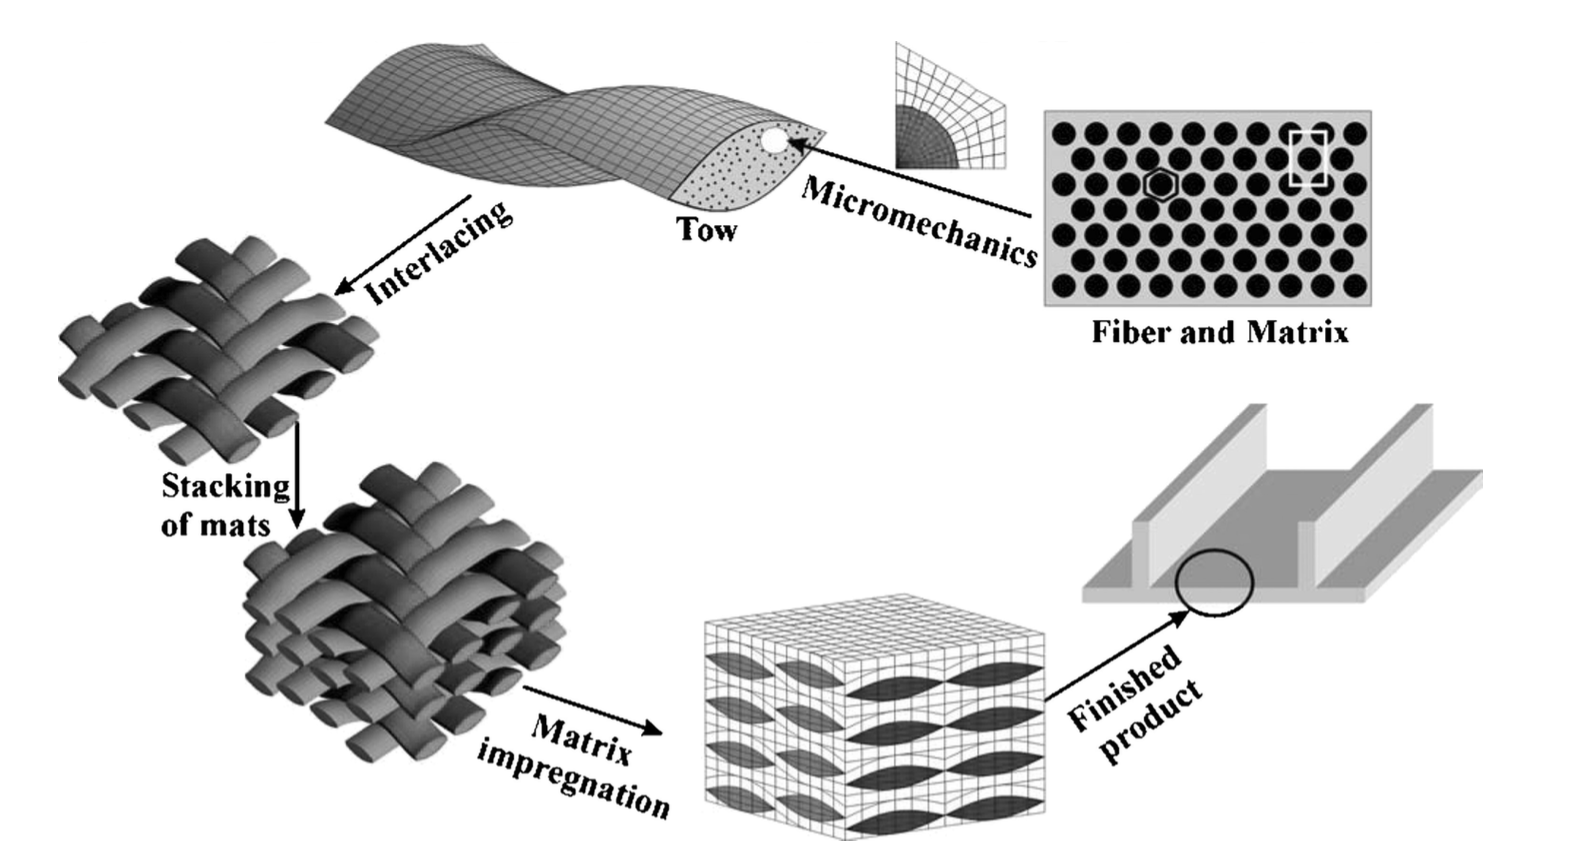
\includegraphics[height=0.25\textheight]{figure/chap1/Goyal}
\fcaption{\citeauthor{Goyal2005}数值模型建立}{\citeauthor{Goyal2005} Numeric Model}
\label{fig:Goyal}
\end{figure*}
对于软管组件的非金属编织加强层,并不包含树脂体系。但是这类编织层的研究少见于文献;事实上,浸润树脂的“硬管”的研究也并不常见:
\citeauthor{Nakai1995}\cite{Nakai1995}分析了编织复合材料管状结构的力学性能,计算了在不产生裂纹的前提下,该结构可承受的最大弯矩和扭矩。
\citeauthor{Leung2013}\cite{Leung2013}发现刚性树脂体系下的管状编织复合材料结构,拉伸至失效,试件编织角变化平均为$ -0.80\textdegree \pm 0.26 \textdegree $ ,甚至要小于工艺控制造成的误差。这显然是“软管”与“硬管”主要的差别,但目前基于符合材料理论的研究,基本没有考虑纤维编织在受力过程中的变化。

\citeauthor{Leung2013}还发现,“硬管”试件编织角发生$ 1\textdegree $的变化,从$ 35 \textdegree$到$ 34\textdegree $,轴向模量上升了近$ 7 \% $;从$ 55 \textdegree$到$ 56\textdegree $,轴向模量并未显著变化。这种轴向模量非线性变化,根据\citeauthor{Ishikawa1982}\cite{Ishikawa1982}应为“偏轴(off-axis)效应”造成的。若没有树脂体系的约束,编织纤维的这种“结构非线性”将会更加明显,也是将来研究的重点。









\section{研究思路}
本研究源于课题《某型PTFE金属编织增强软管组件结构设计原理解析及数值分析》。主要的研究对象为:金属编织增强软管组件的加强层。

  在研究过程中发现,加强层理论的两个分支都经过了数十年的发展,金属纤维缠绕加强,和包含树脂基体的非金属编织加强,这两种加强形式的本构已经形成较为成熟的理论\cite{Evans2002}。
  
 但对于金属纤维编织加强,和无基体或柔性基体的非金属纤维编织加强,目前的理论不能很好的处理\cite{Reese2003}。对这类软管组件的研究,大多沿用钢绞线理论或复合材料理论。两个理论体系并没有太多交集,各有侧重与优势,如表\ref{tab:hose-specimen}所示。

\begin{table}[!htb]
	\centering
	\tcaption{加强层理论体系的比较}{Comparation of Theories of Reiforcement Layers}
	\label{tab:hose-specimen}
	\begin{tabular*}{1.0\textwidth}{@{\extracolsep{\fill}}>{\hspace{0.5cm}}ccc}
		\toprule
		&      钢绞线理论      &  复合材料编织理论   \\\midrule
		着重对象 &       缠绕        &     编织      \\
		研究方法 &     钢丝受力平衡      & 代表性特征单元,平均化 \\
		优势   & \tabincell{c}{考虑结构变化对力学性能的影响} &  \tabincell{c}{考虑复杂结构对力学性能的影响}  \\
		劣势   &     过度简化编织      & 不考虑过程中的结构变化 \\ \bottomrule
	\end{tabular*} 
\end{table}
  
 金属纤维编织加强,和无基体非金属纤维编织加强,有明显的共同点,同时也是研究的难点所在:1.这两种加强形式既包含复杂的纤维间相互作用;2.包含了几何结构明显的变化。对照表\ref{tab:hose-specimen}中两个分支的优势与劣势,恰好需要把两个分支的优势结合起来,才能解决纤维编织加强层的本构问题。
 
 
  
事实上,目前对纤维加强层的理论研究,已经开始有学者试图将这两个方向进行融合:
如\citeauthor{Reese2003}\cite{Reese2003}提出了考虑结构非线性变化的特征单元法;\citeauthor{Rattensperger2003}\cite{Rattensperger2003}利用这种考虑结构非线性的特征单元研究了编织层接头连接扣压的过程。
有学者尝试用连续介质力学的基本理论推导编织层的本构,\citeauthor{Horgan2005}\cite{Horgan2005} 提出了纤维加强材料的应变能密度函数,
国内学者计算了编织结构强度与突加荷载的情况\cite{renjiusheng2009}。
\citeauthor{Wijaya2012}\cite{Wijaya2012}对包含软管各层材料及编织层的试件进行了压缩实验,认为金属编织层的应力应变关系是线性的,在软管整体动态特性的研究中取得了较好的效果。\citeauthor{Cho2005}\cite{Cho2005}研究了编织层在扣压安装接头中的力学行为,结合压缩实验提出了弹塑性的本构模型,\citeauthor{Rattensperger2003}\cite{Rattensperger2003}同样针对压缩的过程,编织层厚度方向引入一组等效非线性弹簧,表征金属纤维间相互作用。
\cite{peirce19375,menges1976spannungs,kato1999formulation,schock1989some,hino1994evaluation}

随着计算机技术的不断发展 ,出现了很多利用有限元计算编织复合材料宏观性能的方法,如\citeauthor{walrath1983losipescu}\cite{walrath1983losipescu}及\citeauthor{hexiaodong1992}\cite{hexiaodong1992}的有限元法,\citeauthor{whyte1986structure}的有限几何模型(FiniteGeometry Model)\cite{whyte1986structure}、有限体胞模型(Finite Cell Model)\cite{chen1999mechanical}、离散有限元素模型(Discrete Finite Element Model) \cite{whitcomb1991},以及庞宝君\cite{pangbaojun2001}针对编织复合材料弹性模量及损伤研究的细观计算力学方法等。


\subsection{Hachemi非线性拉伸模型}

本文希望找到一种模型,可以统一纤维编织加强层的结构非线性,和编织结构微观传力机制的复杂性。
\citeauthor{Hachemi2011}\cite{Hachemi2011}就提出这样一种模型:
建立类似
 \citeauthor{ma_elastic_1986} “对角单元模型”\cite{ma_elastic_1986}的特征单元,单元可以发生大变形,变形的量则是通过钢绞线理论来确定。
 该理论通过特征单元,将编织层的管径,长度联系在一起,相互影响,产生了宏观的非线性力学行为。

 
 \begin{figure*}[!htp]
 	\centering
 	\subfigure{
 		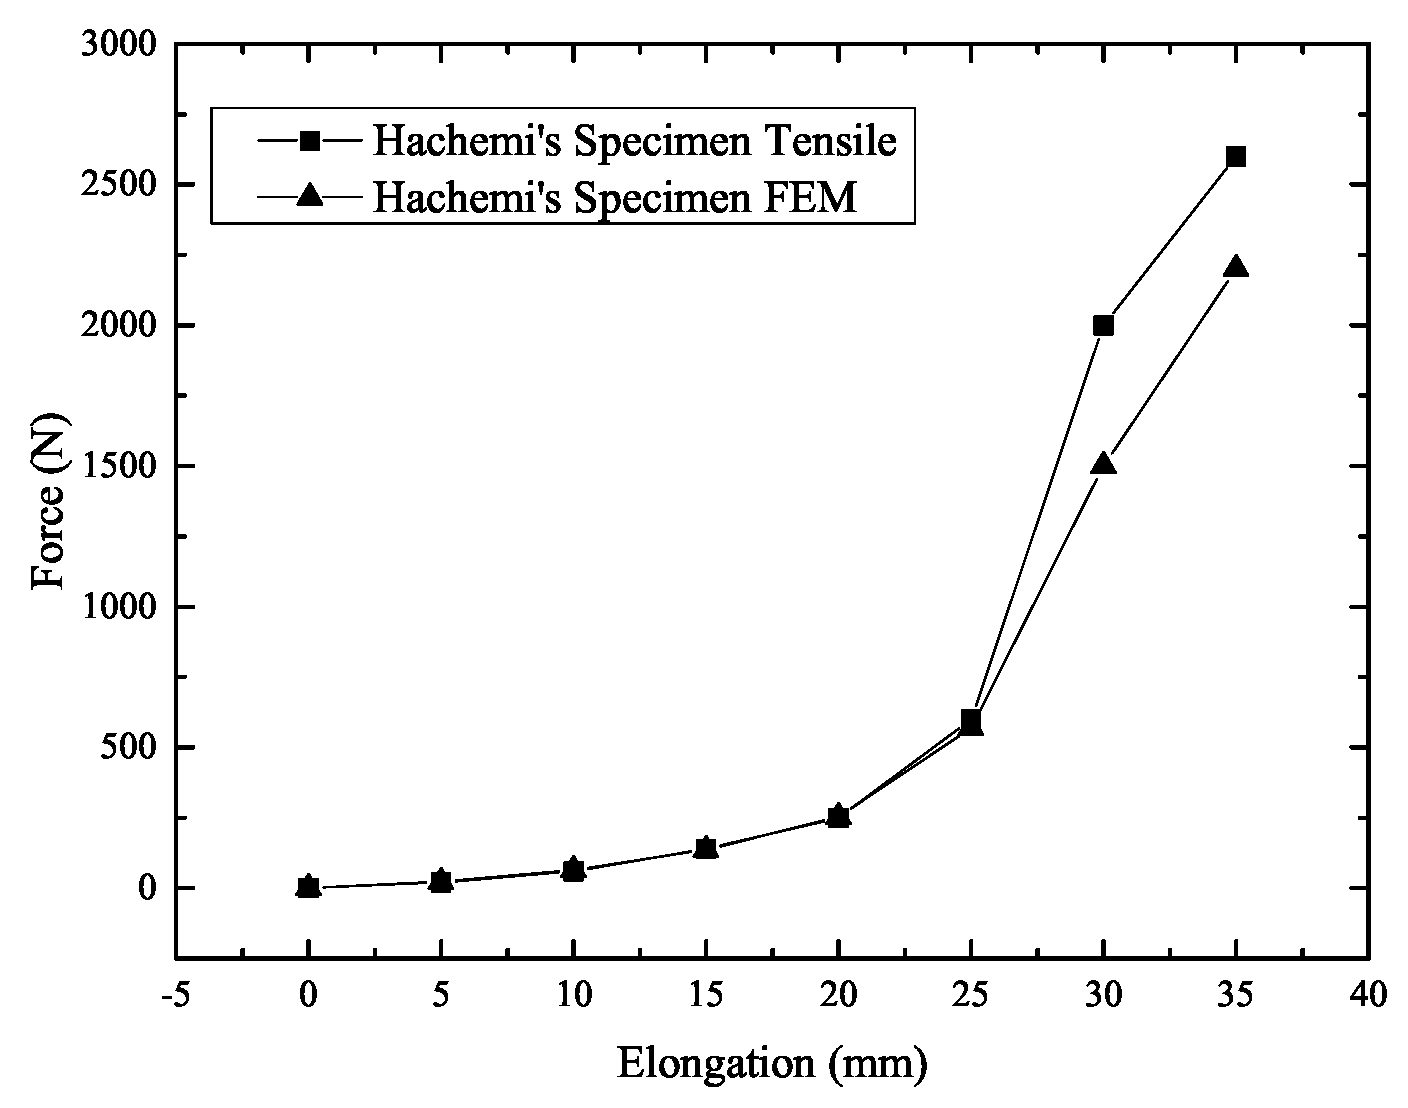
\includegraphics[height=0.22\textheight]{figure/chap1/hachemi}
 		\label{fig:hachemi}
 	}
 	\hspace{1cm}
 	\subfigure{
 		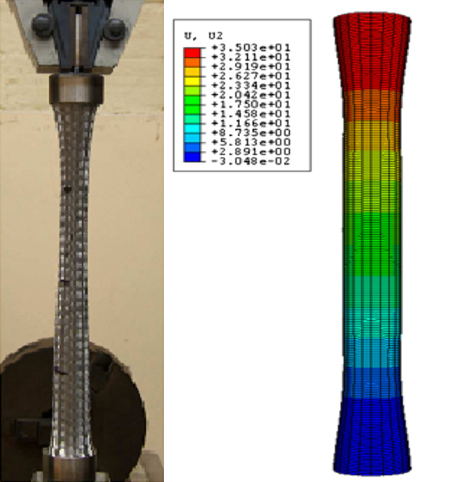
\includegraphics[height=0.21\textheight]{figure/chap1/hachemi-test}
 		\label{fig:hachemi-test}
 	}
 	\fcaption{\ha(2011) 拉伸试验}{Hachemi(2011) tensile experiment}
 \end{figure*}
 
  这种将宏观管体的几何变化与特征单元中细观结构对整体力学行为分开处理的方法值得借鉴但是也较为繁琐,同时\ha 特征单元并未考虑很多对整体的非线性力学行为可能造成影响的因素,还有很大可以改进的空间。因此,本研究将采用这套理论作为研究编织层力学行为的基本构架,并对其进行修改和提升。
 
\citeauthor{Hachemi2011}的这套理论是通过力学万能试验机,对几组金属编织加强层进行了拉伸实验,来验证该模型的。如图\ref{fig:hachemi-test}所示。本研究首先利用较容易实现的拉伸实验验证该模型的有效性,进而发现对于本研究拉伸试验的试件,\ha 模型的非线性行为仍不够强烈。因此本研究开展了多次拉伸实验,围绕改进提升\ha 理论的目标开展研究工作。




 











\section{研究主要内容}
本文可以以软管组件为研究对象,围绕纤维加强层的力学本构的问题,分析了其非线性段的力学行为的结构机理,形成了一套分析方法和
本文主要的研究内容有:
\begin{asparaenum}
	\item 针对软管组件进行了拉伸试验,结合已有的理论,找到了实验中需要关注、记录的关键参数,并针对这些参数,分别设计了测量记录参数的方案。
	\item 根据实验结果与现有理论不吻合的部分,分析了可能导致这种差别的原因,排除了实验误差,挖掘出现有理论提升的空间。
	\item 参考符合材料力学处理编织问题的方法,提出了一套可以解释实验中出现的非线性段力学行为的理论,修正了编织层的刚度,分析讨论理论中各个参数的意义。
	 \item 
	利用准静态的分析方法对软管爆破试验进行了分析,建立了一套可以表针编织层强度的理论。
\end{asparaenum}

本文的研究对象主要是纤维加强层中的编织加强。由于这种结构的复杂性,本文选择现用拉伸实验对编织层的刚度特性进行分析。
拉伸实验中编织层的力位移曲线出现了强烈的非线性特性。
本文认为导致编织结构产生这种非线性现象的原因在于其编织角的变化,类似于结构复杂的非线性弹簧。
针对实验中出现的现象,在现有理论不能合理解释的情况下,本文编织加强层的理论探索就基于该现象展开。


首先,查阅了大量国内外文献,发现Hachemi提出了考虑编织角变化的特征单元法,但是该理论仅能在现行段吻合,原因是该理论并未考虑编织层特有的特性。因此本文的研究就以其理论体系作为基础,展开分析。

确定了研究的基础体系,本文开始对编织层的特性进行分析,剥离处会对力学特性产生影响的因素,提出理论假设和本构模型,形成一套能够解释拉伸实验非线性力位移曲线的理论。

根据理论模型对拉伸实验进行数值仿真,结合实验验证理论的拟合结果。

该结果并不是仅仅针对拉伸实验,而是利用拉伸实验获得的数据,修正理论模型,以此更好地表征编织层的非线性力学行为,进而研究编织层在内压荷载下编织的力学行为,形成编织层的力学理论体系。

本文第一章中,首先对软管组件,软管组件纤维加强层的理论发展进行了回顾和介绍,并提出了本文的研究思路:采用\ha 的编织加强层模型作为基础理论,采用拉伸实验作和数值仿真作为检验手段,对基础模型进行修正,使其能够预报纤维编织加强层非线性的力学行为。

第二章中,详细介绍了软管组件的结构和特性,介绍了软管组件设计生产过程中的重要参数。

第三章,介绍了\ha 模型的基本理论框架,研究了该理论基础下的数值仿真方法。

第四章,对不同规格软管组件进行了拉伸实验,对实验的过程、结果进行了阐述,并分析了实验结果。

第五章,研究了纤维编织加强层中,编织角、纤维间接触、纤维的3维取向等因素对模型非线性段的影响,并分别修正。

第六章,研究了修正后的模型引用与爆破压力实验仿真的效果;研究了将特征单元中,平均化的应力状态转化为纤维应力应变状态的方法,并提出在准静态的数值仿真中得到爆破压力值的方法。

